\chapter{Semi-supervised Learning}
\label{chap:SemisupervisedLearning}

This chapter provides an introduction to and an overview of semi-supervised learning (SSL). The following text draws information predominantly from the article \emph{An Overview of Deep Semi-Supervised Learning} (\cite{SemisupervisedOverview}) and from the book \emph{Semi-supervised learning} (\cite{SslBook}).

In deep learning, the goal typically is to learn some function $f: X \rightarrow Y$ by training a neural network on pairs of data points $(x, y)$. Deep neural networks have large number of trainable parameters, which require adequately large training datasets. Not having enough training data causes the model to overfit and then be unable to generalize to unseen data. Producing training datasets requires a lot of manual labour. Obtaining input data from the domain $X$ is typically easy, the difficult task is assigning correct outputs from $Y$ (called labeling). For this reason, many niche domain problems (e.g. handwritten music recognition or cuneiform recognition) lack sufficiently large labeled datasets for training deep learning models (\cite{MuscimaPP}, \cite{Cuneiforms}). These domains, however, have a relative abundance of unlabeled data.

Semi-supervised learning is a set of methods that aim to utilize this unlabeled data in addition to the available labeled data. The goal of these methods is to produce models that perform better, than models trained on the labeled data alone. The field of SSL has emerged in 1970s and has since accumulated a number of techniques. This thesis focuses on a subset of these techniques, that are based on generative models. However, this chapter provides a short overview of other available techniques as well.

\begin{figure}[p]
    \centering
    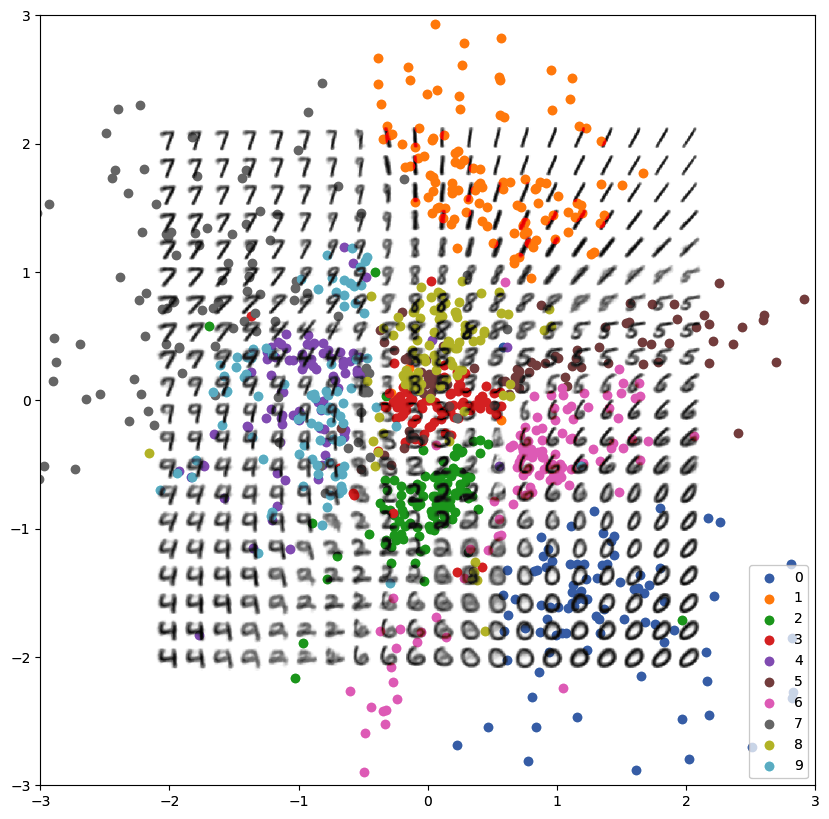
\includegraphics[width=140mm]{../img/mnist-manifold.png}
    \caption{Variational autoencoder learns to project 784-dimensional space of MNIST images down to only 2 dimensional space. We can see clusters of individual classes, forming high-density regions and being separated by low-density regions.}
    \label{fig:MnistManifold}
\end{figure}

\begin{figure}[p]
    \centering
    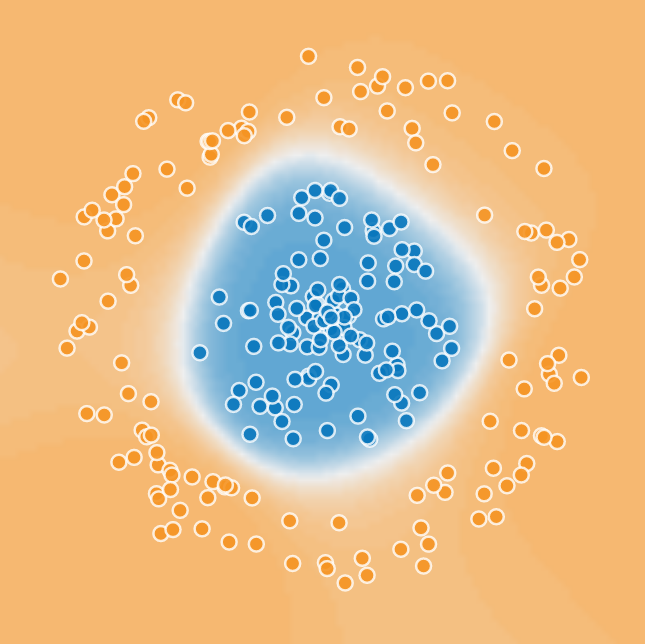
\includegraphics[width=50mm]{../img/decision-boundary.png}
    \caption{Visualization of a classification task, with the decision boundary visible in between the two classes (the while region).}
    \label{fig:DecisionBoundary}
\end{figure}

\qquad

The following text uses a couple of terms, that should be explained first. We will do that on an example:

The figure \ref{fig:MnistManifold} shows the latent space of a variational autoencoder trained on the MNIST dataset (\cite{VariationalAutoencoder}, \cite{Mnist}). The dataset contains grayscale images of handwritten digits, 28x28 pixels in size. In machine learning, the \emph{manifold hypothesis} states, that \emph{real-world high-dimensional datasets lie along low-dimensional manifolds inside that high-dimensional space}. The space of all 28x28 images is such a \textbf{high-dimensional space} (784 dimensions). Manifold, mathematically speaking, is a continuous, locally-eucleidian space (e.g. a plane, sphere, 3D space, Möbius strip). The latent space of the autoencoder is a 2D plane (as seen in the figure \ref{fig:MnistManifold}) and it is the stated \textbf{low-dimensional manifold} containing all the data. The data lies on this manifold, the model has only learned, how this 2D manifold is embeded inside the 784-dimensional space. (Note that it is not the only manifold the data lies on, this is just the one the neural network discovered during training.)

Items of the dataset are not evenly scattered throughout the high-dimensional space. They are coalesced into groups called \textbf{clusters}. Points within these clsuters are located relatively close to each other and usually share the same class. This is an equivalent statement to saying that all digits 7 look alike. These clusters are clearly visible in the latent space (fig. \ref{fig:MnistManifold}), where they form very distinct blobs. The space, where clusters sit, is refered to as \textbf{high-density regions} -- many items from the dataset are located here. Conversely, the space between clusters, where almost no data points are present, is refered to as \textbf{low-density regions}.

A classification task learns a function that assigns a label to each point of the input space. This label is discrete. We can color the input space according to the assigned label and that would produce regions, where all points have the same label. The place where these regions meet is called the \textbf{decision boundary}. A decition boundary can be seen in figure \ref{fig:DecisionBoundary}. In a well-trained classifier for a well-defined classification problem, this decision boundary should lie in the described low-density regions.


\section{Assumptions}
\label{sec:SslAssumptions}

Before we start using semi-supervised methods, we should first understand assumptions that underpin them. These assumptions are mostly intuitive and are satisfied in almost all real-world problems, however stating them explicitly yields better understanding of these methods.

\begin{itemize}
    \item \textbf{The Smoothness Assumption.} \emph{If two points $x_1$, $x_2$ reside in a high-density region and are close together, then their corresponding outputs $y_1$, $y_2$ should also be close together.} For example, if we have a picture of digit 7, then small variations in its shape and color should still be interpreted as digit 7. The opposite statement also holds; if the two input points are separated by a low-density region, the outputs must be distant from each other. This assumption is primarily helpful in a classification task, not so much in a regression task.
    \item  \textbf{The Cluster Assumption.} \emph{If points are in the same cluster, they are likely to be of the same class.} This assumption connects the classification task to the smoothness assumption. It indirectly states, that the decision boundary is located in low-density regions, because otherwise it would cut a cluster in half, causing close points to fall to different classes (which is a violation of the assumption). This assumption can be used as a motivation for methods that push the decision boundary away from data points, into the low-density regions.
    \item \textbf{The Manifold Assumption.} \emph{The (high-dimensional) data lie (roughly) on a low-dimensional manifold.} The problem with high-dimensional data is that as the number of dimensions increases, the volume of the space grows exponentially. This means that most of the space is not covered by any data points in our dataset and that makes it difficult to learn to classify. This assumption states, that our data points actually lie on a small subspace (manifold) of the entire space and that a projection can be learned, that maps this manifold onto a low-dimensional space. Learning the classification task for this low-dimensional space should be much easier.
\end{itemize}


\section{Methods}
\label{sec:SslMethods}

The following section lists major SSL methods. These methods are often directly based on previously stated assumptions and are not mutually exclusive, in fact most of them can be used simultanously as so-called holistic methods. These are, however, not covered in this chapter.


\subsection{Consistency Regularization}

The core idea of this method is that a small neighborhood of each datapoint should have the same label as that datapoint. This idea follows directly from the cluster assumption. In this method we train the model to minimze distance between a known datapoint $x$ and a perturbed datapoint $\hat{x}$. This training is performed in addition to the usual supervised training. This method does not rely on the corresponding label $y$, instead it trains to minimize the distance between $f(x)$ and $f(\hat{x})$. This lets us utilize all unlabeled data points as well.

The method can be seen as an extension of supervised learning. In supervised learning, we train on individual points and learn the overall shape from them. Here, we train on small neighbourhoods, which makes sure the decision boundary will not come close to any individual datapoint. Further utilization of unlabeled data points in the proximity of labeled data points should force the decision boundary even further away, into low-density regions.


\subsection{Proxy-label Methods}

This is a set of methods, that train a supervised model on the labeled data and then use it in some way to label some of the unlabeled data. These methods are also called \emph{bootstrapping}. To distinguish these later-added labels, they are called \emph{pseudo-labels}.

One of these methods is \emph{self-training}. In self-training, labeled data is used to train a supervised classification model. This model is then used to classify all unlabeled data points and since its output is a softmax layer, we can not only pick the most likely class, but also measure the confidence in that class. We define a threshold $\tau$ and only assign pseudo-labels to data points above this threshold. This process can be repeated, until a stopping condition is met (e.g. there are no more unlabeled points with confidence above $\tau$). The main problem of this method is the inability to correct mistakes made during the labeling step.

\emph{Pseudo-labeling} is a similar method, where the unlabeled data points are also assigned pseudo-labels. In this case, these pseudo-labels are treated as trainable parameters, similar to model parameters, and are optimized together with the model during training. The difficult part is designing a good loss function for pseudo-labels, because applying this method naively causes the pseudo-labels to overfit, due to so-called confirmation bias.


\subsection{Graph-based Methods}

These methods frame the problem in the language of graphs. Data points are represented as vertices of a graph and weighted edges are present between pairs of vertices, where the weight corresponds to some similarity between the two points. The labeling task can be viewed as a propagation of information along edges of the graph.

This propagation resembles proxy-label methods, however due to the graph framing, we can consider entities, such as vertex neighbourhood and its impact on the examined node, or we can leverage algebraic structures, like the adjacency matrix.

A different set of graph methods aims to learn data point embeddings, which preserve the structure of the input graph. The goal is to represent each vertex (data point) as a low-dimensional vector, where a simple similarity function (e.g. inner product) would yield similar closeness values as a more complex similarity function in the input space. This again resembles deep learning techniques, such as autoencoding (see figure \ref{fig:MnistManifold}), however here, methods derived from graph theory are used to produce these embeddings (e.g. Laplacian Eigenmaps or Locally Linear Embeddings).


\subsection{Entropy Minimization}

Consistency regularization methods attempt to push the decision boundary away from clusters and into the low-density regions by stabilizing the model output in a neighborhood around each data point. Entropy minimization is a different technique that attempts to do the same thing. In entropy minimization, we penalize the model for being unsure about its predictions. Low-confidence predictions are predictions with more than one class having non-zero probability. Such probability distributions have higher entropy than one-hot distributions. By adding a loss term that minimizes entropy of predictions during training, we can make areas around datapoints more stable. This method can not, however, be used alone for high-capacity models (deep neural networks), as it causes the training to overfit. Instead, it may be used as a supplementing technique to another SSL technique.


\section{Generative Methods}
\label{sec:GenerativeSslMethods}

generative model learns p(x), we then use it to learn p(y|x)
supervised -> add unlabeled
unspuervised -> add labels

\subsection{Variational Autoencoders}

variational autoencoder - kingma et al, M1 M2

\subsection{Adversarial Autoencoders}

adversarial autoencoder

\subsection{Generative Adversarial Networks}

TODO


\section{Related Methods}
\label{sec:RelatedSslMethods}

transfer learning, domain adaptation
    multitask learning
